\lez{4}{02-03-2020}{}
\subsection{Scoperta delle righe (di assorbimento e di emissione).}%
\paragraph{Storia}
Le righe sono state scoperte osservando il sole. Il primo ad osservarle fu Wollaston nel 1802, con la risoluzione che aveva a quei tempi vide 5 intense bande scure e 2 bande scure più deboli. Lui attribuì a tali linee il ruolo di demarcazione tra lo spettro dei colori fondamentali sbagliando alla grande. \\
Qualche anno dopo Fraunhofer riuscì a vederne tandissime \footnote{Inventandosi uno spettroscopio molto preciso.}, a quelle più intense diede nomi dalla A alla H (ancora usate) oggi, fu quindi chiaro che queste non potevano essere le linee di demarcazione tra i colori fondamentali.\\
Fraunhofer si mise allora ad osservare le altre stelle più luminose (come Sirio), scoprendo in larghissimo anticipo che anche queste mostravano delle righe di assorbimento e noto che le lrighe presenti in sirio non erano le stesse di quelle osservate nel sole. \\
Sempre lui osservando i pianeti si accorse che questi presentavano le stesse righe presenti nel sole \footnote{Adesso sappiamo che questo è dovuto allo scattering della luce solare sulla faccia del pianeta.}. \\
Il grande intuito di Fraunhofer non si fermo ancora, egli fù capace di osservare che la linea scura da lui nominata D sembrava coincidere con il doppietto delle righe luminose presenti nelle lampade al sodio.\\
Oggi Fraunhofer è considerato l'inventore della Spettroscopia astronomica, le sue osservazioni sono tra le più importanti in questo campo scientifico.\\
Dopo 30 anni Focault volle verificare la coincidenza della riga di emissione delle lampade al sodio con quella di assorbimento del sole D. Per farlo fece passare la luce del sole attraverso un gas di sodio scaldato e ne misurò lo spettro. Focault si aspettava che gli effetti di assorbimento e di emissione si compensassero dando luogo ad un continuo di fatto. \\
Quello che successe invece è che lo spettro della luce del sole che attraversa il gas non solo pesentava le righe di assorbimento ma queste risultarono addirittura accentuate. Fece inoltre passare una luce a spettro continuo prodotta con un corpo incandescente attraverso lo stesso il gas di sodio, anche in questo caso vide le righe nere.\\
Per altri dieci anni tutto tace fino all'arrivo di un fisico teorico tedesco: Kirchhoff. Egli riprese gli esperimenti citati sopra e formulo tre famose leggi: 
\begin{fact}[Leggi di Kirchhoff]{fact:Leggi di Kirchhoff}
	\begin{enumerate}
		\item Tutti i corpi incandescenti producono uno spettro continuo.
		\item Un gas rarefatto caldo emette delle righe di emissione.
		\item Preso un gas rarefatto su cui facciamo incidere della radiazione con spettro continuo otteniamo 
			\begin{itemize}
				\item Se la radiazione emessa è meno intensa della radiazione che retroillumina ($s_{\nu} < I_{\nu} ( 0) $ ): righe di assorbimento.
				\item Se la radiazione emessa è più intensa della radiazione che retroillumina ($s_{\nu} > I_{\nu} ( 0) $ ): righe di emissione.
			\end{itemize}
	\end{enumerate}
\end{fact}
Nella nostra formulazione la terza legge deriva dalla soluzione all'equazione del trasporto per un mezzo omogeneo nella \ref{eq:soluzione-mezzo-omogeneo}.
\[
	I_{\nu} ( \tau _{\nu} ) = I_{\nu} ( 0)e^{-\tau _{\nu} } + s_{\nu} \left( 1-e^{-\tau _{\nu} } \right) 
.\] 
Se il mezzo è otticamente sottile questa può essere approssimata:
\[
	I_{\nu} ( \tau _{\nu} ) \approx I_{\nu} ( 0) -\tau _{\nu} I_{\nu} ( 0)  + s_{\nu} \tau _{\nu} = I_{\nu} ( 0) + \tau _{\nu} ( s_{\nu} -I_{\nu} ( 0) ) 
.\] 
Quindi oltre al fondo della sorgente si vedono righe di emissione o di assorbimento a seconda del segno del secondo termine \footnote{Di fatto $s_{\nu} $ inserisce o rimuove le righe degli atomi che compongono il mezzo rarefatto dallo spettro continuo della radiazione.}. \\
Ne seguì l'intuizione che un mezzo è in grado di emettere soltanto le frequenze che è anche in grado di assorbire.\\
In questo modo Kirchhoff e Bunzen ricominciarono ad osservare il sole e allo stesso tempo le righe di emissione di alcuni elementi sulla terra capendo che nel sole erano presenti Sodio, Nichel, Ferro, ecc\ldots\\
Si aprì così una finestra allo studio della composizione chimica delle stelle, questa fu una grande smentita per il filosofo Compte che in preda a delirio di preveggenza disse che:
\begin{center}
	"Of all objects, the planets are those which appear to us under the least varied aspect. We see how we may determine their forms, their distances, their bulk, and their motions, but we can never known anything of their chemical or mineralogical structure; and, much less, that of organized beings living on their surface ..." \\
	\null\hfill Auguste Comte, The Positive Philosophy, Book II, Chapter 1 (1842) 
\end{center}
Infatti fu prontamente smentito dai suoi coetanei scienziati \footnote{Chissà se forse questo sarà il baluardo di ogni genere di Teologia, costretta a riplasmare ogni affermazione fino all'osso a causa dell'inarrestabile potenziamento delle conoscienze umane.}.\\
Abbiamo comunque un importante risultato per la spettroscopia: la presenza di righe di assorbimento di un elemento in uno spettro mi garantisce che nella regione di provenienza di tale spettro vi è l'elemento corrispontente a tali righe.\\
Si scoprì più avanti che in uno spettro non vi sono soltanto informazioni sulla composizione chimica degli elementi della sorgente: abbiamo anche l'abbondanza dell'elemento rispetto agli altri, le condizioni fisiche dell'atmosfera in cui si forma una riga. \\
\subsection{Radiazione di corpo nero: proprietà principali.}%
Prima di ricavare la forma della $s_{\nu} $ è necessario ricordare alcuni concetti importanti sul corpo nero.\\
Kirchhoff dimostro con la sua prima legge che la radiazione di un corpo all'equilibrio termodinamico ha uno spettro indipendente dalle proprietà fisiche del mezzo stesso.
\begin{fact}[Radiazione all'equilibrio termodinamico con la materia]{fact:Radiazione all'equilibrio termodinamico con la materia}
	Lo spettro della radiazione all'equilibrio termodinamico con la materia è una funzione universale della temperatura.
\end{fact}
Kirchoff non riuscì a trovare la $I_{\nu} $ corrispondente a tale radiazione, ci fù bisogno di Plank che ricavò la radiazione di corpo nero come:
\begin{defn}[Radiazione di corpo nero]{def:Radiazione di corpo nero}
	La radiazione all'equilibrio termodinamico con la materia di un corpo può essere espressa come:
	\[
		I_{\nu} = B_{\nu} = \frac{2\hbar }{c^2} \frac{\nu ^3}{\exp\left( \frac{\hbar\nu }{kT} \right) -1}
	.\] 
	Questa è definita come la radiazione di corpo nero.
\end{defn}
È necessario ricordare alcune proprietà di questa radiazione. Partiamo dalla forma:
\begin{figure}[H]
	\centering
	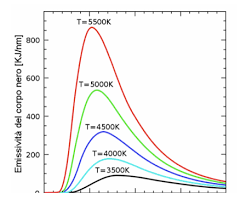
\includegraphics[width=0.2\textwidth]{figures/plank.png}
	\caption{\scriptsize Piccola immagine della funzione per vari valori della temperatura.}
	\label{fig:figures-plank-png}
\end{figure}
\paragraph{Legge di spostamento di Wien}
Al crescere di T il picco si sposta verso destra secondo la legge:
\[
	h \nu _{\text{max}} \propto kT
.\] 
In astrofisica conviene riportarla in termini di lunghezza d'onda $\lambda$:
\[
	\lambda _{\text{max}}T = 0.29 \left[ \text{cm} \right]\cdot  \left[ \text{K} \right] 
.\] 
Dobbiamo stare attenti al fatto che $\lambda _{\text{max}}$ non è il massimo della $B_{\nu} $, bensì è il massimo della $B_{\lambda} $ è quindi necessario cambiare variabile alla funzione per la radiazione di corpo nero, per farlo basta:
\[
	I_{\nu} d\nu = I_{\lambda } d\lambda 
.\] 
Per aiutare la memoria nel passaggio tra le due forme possiamo ricordare il caso del sole: la temperatura superficiale del sole è $T \approx 6000$ K, in questo caso abbiamo che  $\lambda _{\text{max}} \approx 5000$ \AA $ \ $ e quindi abbiamo emissione nel visibile.
\paragraph{Densità di energia del corpo nero}
\[
	u_{\nu} ( T) = \int \frac{I_{\nu} }{c}d\Omega = \frac{4\pi}{c}B_{\nu} ( T) 
.\] 
Su tutto lo spetttro si ha:
\begin{align}
	u =& \int u_{\nu} d\nu =\\
	=& \int \frac{4\pi}{c} B_{\nu} ( T) d\nu =\\
	=& \frac{4\pi}{c}\frac{2\hbar }{c^2} \int \frac{\nu ^3}{\exp\left( \frac{h \nu }{kT} \right) -1}d\nu = \\
	=& \frac{8\pi^{5}k^{4}}{15c^3h^3}\cdot T^{4} = a \cdot T^{4}
.\end{align}
Dove si è usato l'integrale noto:
\[
	\int \frac{x^3}{e^{x}-1}dx = \frac{\pi^{4}}{15}
.\] 
\subsection{Temperatura di una stella}%
Dobbiamo decidere le convenzioni da adottare per la misura della temperatura di una stella. La questione è davvero complessa, la stella è un oggetto dalle caratteristiche non uniformi, basti pensare alla sua densità che varia da qualche frazione inferiore a quella dell'aria a decine di volte quella dell'acqua. \\
Inoltre per questi oggetti non è nemmeno possibile definire una superficie, quindi dove misuriamo la temperatura? Per concludere il quadro già complesso dobbiamo pensare che l'unica fonte di informazioni a nostra disposizione sono le radiazioni che ci arrivano dalle stelle, quindi dovremmo estrarre l'informazione Temperatura da queste.
\paragraph{Temperatura di Brillanza.}
e misuriamo l'intensità specifica monocromatica di una sorgente $I_{\nu} $ possiamo definire la temperatura di Brillanza:
\begin{defn}[Temperatura di brillanza]{def:Temperatura di brillanza}
	Data un oggetto avente brillanza $I_{\nu} $ la sua temperatura di brillanza $T_{B}$ è la temperatura che ha un corpo nero che alla frequenza $\nu $ emette la stessa intensità specifica $I_{\nu} $.
	\[
		I_{\nu} = B_{\nu} ( T_{B}) 
	.\] 
\end{defn}
Una conseguenza diretta di questa definizione è che la temperatura di un oggetto sarà diversa a seconda della frequenza misurata (anche dello stesso oggetto). \\
Questa temperatura è molto utile in radio-astronomia, in tal caso siamo nel regime di Rayleigh-Jeans:
\[
	h \nu  \ll kT
.\] 
Quindi possiamo espandere la $I_{\nu} $ ottenendo:
\[
	I_{\nu} = B_{\nu} ( T_{B}) \approx \frac{2\nu ^2}{c^2}kT_{B}
.\] 
A questo punto possiamo ricordare la forma della equazione del trasporto:
\[
	\frac{\mbox{d} I_{\nu} }{\mbox{d} \tau _{\nu} } = s_{\nu} -I_{\nu} 
.\] 
Prima di procedere è necessario notare che radiazione termica e radiazione di corpo nero sono due cose distinte: la radiazione termica si ha quando l'oggetto che emette è all'equilibrio termodinamico con la radiazione, la radiazione termica diventa quella di corpo nero quando il mezzo che emette diventa otticamente spesso.\\
\begin{fact}[Legge di Kirchhoff]{fact:Legge di Kirchhoff}
	Per un mezzo all'equilibrio con la sua radiazione termodinamica si ha $s_{\nu} = B_{\nu} $.
\end{fact}
Per dimostrarla mettiamoci all'interno di un corpo nero cavo: la radiazione di corpo nero è omogenea e isotropa, quindi in questo ambiete si ha:
\[
	\frac{\mbox{d} I_{\nu} }{\mbox{d} \tau _{\nu} } = 0 
.\] 
Quindi si ha che $s_{\nu} = I_{\nu} $, ma nel caso di corpo nero $I_{\nu} = B_{\nu} $, quindi si ottiene quanto atteso: $s_{\nu} = B_{\nu} $.\\
Possiamo quindi riprendere l'utilità della temperatura di brillanza, prendiamo un oggetto all'equilibrio termodinamico avente temperatura di brillanza $T_{B}$ e temperatura del mezzo $T$, sostituiamo tutte le quantità all'interno dell'equazione del trasporto (considerando anche la legge di Kirchhoff):
\[
	\frac{\mbox{d} }{\mbox{d} \tau _{\nu} }\left( \frac{2\nu ^2}{c^2}kT_{B} \right) = \frac{2\nu ^2}{c^2}kT -  \frac{2\nu ^2}{c^2}kT_{B} 
.\] 
Adesso semplifichiamo tutte le costanti, ci resta una semplice equazione differenziale lineare in $T_{B}$:
\[
	\frac{\mbox{d} T_{B}}{\mbox{d} \tau _{\nu} } = T -T_{B}
.\] 
quindi possiamo risolvere come abbiamo fatto per l'equazione del trasporto:
\[
	T_{B}( \tau _{\nu} ) = T_{B}( 0) e^{-\tau _{\nu} } + \int_{0}^{\tau _{\nu} } T( \tau _{\nu} ')e^{-\left( \tau _{\nu} -\tau _{\nu} ' \right) } d\tau _{\nu} ' 
.\] 
A questo punto se il mezzo è omogeneo possiamo fare gli stessi passaggi già fatti per ottenere:
\[
	T_{B}( \tau _{\nu} ) = T_B( 0) e^{-\tau _{\nu}} + T \left( 1-e^{-\tau _{\nu} } \right) 
.\] 
Quindi se la radiazione emerge da un mezzo spesso si ha che:
\[
	T_{B} \approx T
.\] 
Per questo nel limite di Rayleigh-Jeans la temperatura di brillanza è utile, perchè è una ottima approssimazione della temperatura del mezzo.\\
Nel limite opposto, quindi $h \nu \gg kT$ si avrà:
\[
	I_{\nu} \approx \frac{2\hbar \nu ^3}{c^2}\exp\left( - \frac{h \nu }{kT} \right) 
.\] 
Di conseguenza l'equazione di trasporto smette di essere lineare, quindi il concetto di temperatura di brillanza non è comodo qui. Ad esempio se si osserva nel $\gamma $ non si usa la temperatura di brillanza.
\paragraph{Temperatura di colore}
Quando non si conosce l'intensità specifica ma si conosce lo spettro della radiazione raccolta, ovvero il flusso della radiazione raccolta sulla terra.
Questo può essere il caso di un'oggetto di cui non sappiamo le dimensioni e non sappiamo la distanza.
\begin{defn}[Temperatura di colore]{def:Temperatura di colore}
	Si definisce la temperatura di colore come la temperatura che avrebbe un corpo nero il cui picco si trova nella stessa posizione in frequenza del picco dello spettro che stiamo osservando.
\end{defn}
Questa definizioe si rifà di fatto all'uso della legge di spostamento di Wien per formulare una previsione sulla temperatura.
\paragraph{Temperatura effettiva}
Questa è la più utilizzata quando parliamo di temperatura superficiale di una stella.
\begin{defn}[Temperatura effettiva]{def:Temperatura effettiva}
	La temperatura effettiva è la temperatura di un corpo nero tale che:
	\[
		\Phi_{\text{corpo nero}} = \Phi_{\text{Osservato}}
	.\] 
\end{defn}
Quindi ci serve di conoscere il flusso intrinseco della radiazione. Ci serviranno per questo la distanza e le dimensioni dell'oggetto.\\
Vediamo come sono legate l'intensità $L$ intrinseca della sorgente al raggio dell'oggetto: \\
Prendiamo una sorgente sferica di raggio $R$ e di luminosità intrinseca $L$ abbiamo che
\[
	F = \frac{L}{4\pi R^2}
.\] 
Ma il flusso è anche uguale a: $F = \sigma T^{4}$ per la legge di Stephan-Boltzmann. Quindi questo ci permette di definire la temperatura effettiva:
\[
	L = 4\pi R^2 \sigma T_{\text{eff}}^{4}
.\] 
La temperatura effettiva è legata alla radiazione che emerge da un certo strato della stella, da questo strato vedremo che proviene gran parte della radiazione che osserviamo. Il motivo è che a lunghezze d'onda differenti corrispondono coefficienti di assorbimento differenti, quindi i fotoni scapperanno dalla stella a "profondità diverse".\\
Lo strato atmosferico da cui proviene gran parte della radiazione è chiamato fotosfera, vedremo che la temperatura effettiva proviene da un certo punto della fotosfera.
\subsection{Cammino libero medio dei fotoni}%
Abbiamo visto che per un mezzo assorbente $j _{\nu} = 0$ abbiamo 
\[
	I_{\nu} ( \tau _{\nu} ) = I_{\nu} ( 0) e^{-\tau _{\nu} }
.\] 
Ci chiediamo adesso qual'è la probabilità che un fotone di frequenza $\nu $ riesca ad attraversare nel mezzo una profondità ottica almeno pari a $\tau _{\nu} $. Questa sarà data evidentemente dalla equazione scritta sopra:
\[
	P_{\text{abs}} = e^{-\tau _{\nu} }
.\] 
Possiamo calcolarci quindi la profondità ottica media:
\[
	\left< \tau _{\nu}  \right> = \int_{0}^{\infty} \tau _{\nu} e^{-\tau _{\nu} } d\tau _{\nu} = 1 
.\] 
Se siamo in un mezzo omogeneo abbiamo che $\tau _{\nu} = \alpha _{\nu} l_{\nu} $, abbiamo quindi il cammino libero medio, definito come:
\begin{defn}[Cammino libero medio]{def:Cammino libero medio}
\[
	l_{\nu} = \frac{1}{\alpha _{\nu} }
.\] 
\end{defn}
Se il mezzo non è omogeneo si calcola il valore del cammino libero medio che il fotone avrebbe in un mezzo omogeneo con le proprietà fisiche che ha in quel punto.\\
Vediamo che il cammino libero medio dipende pesantemente dalla frequenza, quindi i fotoni che ci arrivano da una stella arrivano da una corona circolare poichè ogni frequenza avrà cammino libero medio differente \footnote{Ad esempio le frequenze nei pressi di una riga di assorbimento saranno emesse più in superficie.}.

\subsection{Equilibrio termodinamico locale}%
È possibile utilizzare il concetto di cammino libero medio per definire il concetto di equilibrio termodinamico locale. Infatti se la temperatura in un corpo resta costante su scale dell'ordine del cammino libero medio allora la deviazione dalla condizione di equilibrio termodinamico sarà piccola ed avrà senso parlare di equilibrio termodinamico locale (LTE).\\
Spesso ci capiterà di metterci in situazioni di LTE poichè sono molto comuni in mezzi che studieremo nel cosmo.\\
Ad esempio all'interno della stella abbiamo in genere un cammino libero medio microscopico, quindi qui avrà senso porci in condizioni di LTE, sulla superficie esterna di una stella invece no. \\
Quindi in una regione di LTE è possibile assumere che le particelle abbiano distribuzione di velocità secondo Maxwell, gli atomi abbiano popolazioni dei livelli secondo Boltzmann e vale la legge di Kirchhoff. 
